\documentclass[11pt,a4paper]{article}

\usepackage[utf8]{inputenc}
\usepackage[T1]{fontenc}
\usepackage{lmodern}
\usepackage[margin=2.5cm]{geometry}
\usepackage{amsmath,amssymb}
\usepackage{graphicx}
\usepackage{float}
\usepackage{url}
\usepackage[hidelinks]{hyperref}

\graphicspath{{figures/}}
\setlength{\parskip}{0.6em}
\setlength{\parindent}{0pt}

% let long URLs break after / and -
\expandafter\def\expandafter\UrlBreaks\expandafter{\UrlBreaks\do\/\do\-}

% headings: "I] INTRODUCTION" and "1. Title" (italic, underlined)
\makeatletter
\renewcommand{\thesection}{\Roman{section}]}
\renewcommand{\thesubsection}{\arabic{subsection}.}
\renewcommand{\@seccntformat}[1]{\csname the#1\endcsname\hspace{0.5em}}
\renewcommand{\section}{\@startsection{section}{1}{0pt}{1.4em}{0.6em}{\normalfont\bfseries}}
\renewcommand{\subsection}[1]{\@startsection{subsection}{2}{0pt}{1em}{0.4em}{\normalfont\itshape}{\underline{#1}}}
\makeatother

% reference list with hanging indent
\newenvironment{references}{\sloppy\list{}{\leftmargin=1.5em \itemindent=-1.5em \itemsep=0.3em \parsep=0pt}}{\endlist}

\begin{document}

\begin{center}
  {\large\bfseries Descriptive Representation Without Executive Power: The Incomplete Effects of Gender Quotas}
\end{center}

\section{INTRODUCTION}

In 1995, in France, women represented only 22\% of municipal councillors and 7\% of mayors (Lippmann, 2018). This prompted the adoption of the 2000 ``Loi sur la parité'' imposing parity on candidate lists. At the municipal level, the law was first applied to municipalities with over 3,500 inhabitants in the 2001 elections, before it was strengthened into a zipper quota, mandating strict gender alternation on candidate lists, and extended to require parity within elected deputy mayors (``adjoints au maire'') in 2008 elections. Finally, in 2014, both the zipper quota and the deputy mayor parity requirement were extended to municipalities above 1,000 inhabitants, leaving the mayoral position as the only level in the hierarchy unconstrained by gender requirements.

While these reforms were successful at mechanically increasing the number of women on candidate lists, their broader effects on women's access to leadership positions remain contested. This suggests the persistence of barriers preventing women from reaching top political positions, reflecting a potential ``glass ceiling'' effect (Lippmann 2018). Regarding French municipal elections, Lippmann argues that quotas are ineffective at breaking this glass ceiling, but rather simply raise it to the legally mandated level. Lassébie (2020) also provides empirical evidence supporting this claim, showing that zipper quotas significantly increased the share of female municipal councillors but had no effect on the share of female mayors. Similar results were found by Spaziani (2022) in Italy, who showed that gender quotas increased female representation in less ``senior government positions'' but produced no effect on mayoral positions. However, O'Brien and Rickne (2016) delivered a more optimistic picture from Sweden municipalities, showing that municipalities where the zipper quota had a larger impact on women's descriptive representation became significantly more likely to select female party leaders. Following these considerations, we seek to determine the effect of quotas on women's access not only to councillor and mayoral positions, but also to the intermediate executive position of deputy mayor. We thereby want to test where the glass ceiling effect lies.

Moreover, the historically increasing presence of women in politics provides ground for theories pointing to a ``role model effect'', stating that the presence of women in leadership positions reduces bias against female candidates and improves their prospects in future elections (Beaman et al. 2009). This effect is identified across different settings: in the US, the presence of a female office holder is shown to be a motivating factor significantly increasing women candidates (Ladam et al. 2018); in Switzerland, the previous increase in elected women in nearby municipalities pushed more women to run for office (Gilardi 2015); in India, women are more likely to run and be elected in councils previously led by a woman (Beaman et al. 2009). Building on this framework, we will examine whether female mayors act as a catalyst for increased female representation in the French municipal context.

This paper therefore contributes to the literature on gender quotas and political representation in three ways. First, we extend the analysis beyond the councillor and mayor dimensions by introducing deputy mayors, contributing to the mapping of where the glass ceiling lies. Second, by implementing a Difference-in-Discontinuities design across three electoral cycles, we assess not only the immediate impact of the 2013 reform but also how its effects persist over time. Third, we provide a test of whether the quota effect varies with prior female leadership context, contributing to the broader debate on role model dynamics.

\section{INSTITUTIONAL BACKGROUND}

Our study focuses on French municipalities, which are the basic unit of local government in France, and are governed by municipal councils elected every six years by direct universal suffrage. Their size is determined by the population of the municipality, ranging from 7 to 69 seats. Following each election, the elected representatives convene to elect a mayor and deputy mayors (\textit{adjoint au maire}) among its members. Mayors hold the main executive authority, acting as the representative of the State at the local level, and as head of the municipal executive. Deputy mayors are delegated specific policy responsibilities and constitute the municipal executive. The remaining representatives of the municipal council are councillors.

Municipal elections follow different rules depending on population size. In municipalities below 1,000 inhabitants, elections were based until 2026 on a plurality system with individual candidates. In municipalities above 1,000 inhabitants, elections follow a two-round proportional system with closed lists, and seats are allocated proportionally after a majority bonus is awarded to the winning list.

The \textit{Loi sur la parité} of 2000 imposed gender parity requirements on candidate lists for a range of elections. It required that candidate lists be composed of 50\% women, both overall and within each block of six candidates to prevent strategic concentration of women to unelectable positions. This first applied to municipalities above 3,500 inhabitants in the 2001 elections. Between 2001 and 2008, the law was strengthened, the block-based rule was replaced by strict alternation between male and female candidates (zipper quota), eliminating the possibility to cluster women in less prominent positions. Additionally, the parity requirement was extended beyond candidate lists to include the composition of the deputy mayor group. Then, in 2013, the population threshold for the application of quota was lowered to 1,000 inhabitants, and became effective for the 2014 elections. (Vie Publique, 2026) This extension is the quasi-experimental variation we exploit in this paper.

\section{DATA SOURCES}

The main data source for this project comes from the Répertoire National des Élus (RNE), which centralises information on elected politicians' name, gender, occupation, and type of mandate. The publicly available version, provided by the Ministère de l'Intérieur, covers all elected representatives as of December 2025, therefore encompassing the 2020-2026 municipal mandate. Data for previous mandates has been recovered from the Base Révisée des Elu.es de France (BRÉF), a database elaborated from historical RNE data describing the mandates of all elected representatives during the Fifth Republic.

From these sources, we recovered data on mayors dating back to 2001, and on other members of the municipal council since 2008. We will focus on officials elected during the national rounds of municipal elections in metropolitan France (March 2001, March 2008, March 2014, March and June 2020). A potential limit of our data is that it is liable to misrecording or misreporting of different roles in the municipal council. To mitigate this concern, we focus our analysis on periods with more consistent reporting and fewer missing values. Therefore, because of the lack of information on the majority of the municipal council, we restrict our use of 2001 data to the mayoral level. Similarly, we begin our analysis of deputy mayors in 2014, as the distinction between municipal councillors and deputy mayors was reported by only a limited number of municipalities in 2008.

We then aggregated the data at the municipal level, considering the gender of the mayor and computing the proportion of women in the municipal council, and in each of the functions of councillors and deputy mayors. Focusing on municipalities with under 10,000 inhabitants, our dataset contains information about 35654 municipalities in 2008, 35637 in 2014, and 32955 in 2020, therefore representing over 95\% of all French municipalities.

Additionally, we used INSEE data to recover municipal characteristics, including unemployment, age and sex distribution, PCS, and population. Population being our running variable, we have used for each electoral year the reference population for electoral matters (1999 authenticated population for 2001 and 2008 elections, 2011 for 2014, 2017 for 2020).

\section{EMPIRICAL STRATEGY}

\subsection{Identification Strategy and Difference-in-Discontinuities Design}

To estimate the effect of electoral quotas on female political representation across the municipal hierarchy, we exploit the changing scope of the French Parity Law, which was extended in 2014 from municipalities with more than 3,500 inhabitants to those with more than 1,000 inhabitants. This reform generates a sharp discontinuity in the application of electoral gender quotas at the 1,000 inhabitant threshold, which we exploit using a Regression Discontinuity Design (RDD). The underlying assumption is that municipalities just above and below the 1,000 inhabitant threshold are comparable, so that discontinuity at the cutoff can be attributed to the quota policy rather than underlying differences, which we verify by testing for continuity of covariates at the threshold.

However, a simple RDD at the threshold would confound the effect of quotas with the effect of other institutional rules at the cutoff, notably the electoral system (shifting from plurinominal majority voting to a proportional closed-list system), as well as salaries of mayors. Moreover, we performed a McCrary test for each year and found evidence of population sorting around the 1,000 inhabitant cutoff. Following the approach taken by Bagues and Campa (2016) and Lassébie (2019), we implement a Difference-in-Discontinuities design, comparing the size of the discontinuity in outcomes at the 1,000 inhabitant threshold across elections.

In 2008, no municipality near this threshold was subject to the parity law, so that any discontinuity in outcomes at the cutoff captures the effect of the confounding institutional rules and sorting. By differencing the discontinuity observed in the post-reform periods (2014 and 2020) from that in the pre-reform election, we recover the causal impact of the quota policy, under the assumption that confounding policies and manipulation remained stable over time. Additionally, we reduced our sample to municipalities who do not change treatment status, to avoid capturing the effect of municipalities becoming treated.

Formally, we estimate separate local linear regressions for each period \textit{t} $\in$ \{2008, 2014, 2020\}:
\[
Y_{it} = \alpha_{t} + \beta_{t}D_{i} + f_{t}(pop_{i} - 1000) + \varepsilon_{it}
\]
where $Y_{it}$ is the outcome of interest for municipality $i$ in election year $t$, $pop_{i}$ is the municipality's population, $D_i = \mathbf{1}[pop_{i} > 1000]$ is our treatment indicator, and $f_{t}(pop_{i} - 1000)$ a polynomial capturing the relationship on either side of the threshold.

\subsection{Implementation by outcome}

We apply our design over the municipal hierarchy. For councillors and mayors, data are available across all electoral waves, and we use 2008 as the pre-reform placebo period and 2014 and 2020 successively as the post-reform periods. Our difference-in-discontinuities estimators are then : $\delta_{1} = \hat{\beta}_{2014} - \hat{\beta}_{2008}$ and $\delta_{2} = \hat{\beta}_{2020} - \hat{\beta}_{2008}$. Comparing both post-reform waves allows us to assess whether the effect of quotas accumulates over electoral cycles.

For deputy mayors, the position was not systematically recorded in the RNE before 2014, so that we don't have a reliable pre-reform observation from this outcome. We therefore present simple RDD estimates for 2014 and 2020 separately. Their interpretation must be thus nuanced, and can only be seen as an upper bound for the impact of quotas.

\subsection{Estimating the role model effect}

If a role model effect exists, so that the pool of female candidates and the willingness of voters to select them is increased by exposure to female political leadership, we postulate that gender quotas should be more effective (generating a greater increase in female representation) in municipalities where women were already visible in leadership roles. To investigate the role model effect, we extend the difference-in-discontinuities framework to study the heterogeneous effect of quotas across subsamples on two dimensions of female political context.

First, we consider heterogeneity by previous female mayor, splitting municipalities according to the gender of the previous mayor, and estimate the difference-in-discontinuities on each. Concretely, for each subsample \textit{s} $\in$ \{previous female mayor, no previous female mayor\}, we estimate: $\beta_{1}^{s} = \hat{\delta}_{2014}^{s} - \hat{\delta}_{2008}^{s}$ where $\hat{\delta}^{s}$ is the RD coefficient estimated on subsample \textit{s} in year \textit{t}. Evidence of a role model would correspond to $\hat{\beta}_{1}$\textit{\{previous female mayor\}} $>$ $\hat{\beta}_{1}$\textit{\{no previous female mayor\}}.

Secondly, to capture the broader political environment of neighbouring municipalities, we construct for each municipality the share of female mayors in its department in the previous mandate, excluding the municipality itself. We then split the sample into terciles (low, medium, and high female leadership contexts) and estimate the difference-in-discontinuities separately on each subsample. This tests whether the causal effect of gender quotas varies with the degree of political feminisation in surrounding municipalities.

A limit regards the comparability of the subsamples, as municipalities that previously elected a female mayor might differ from other municipalities on unobservable dimensions such as local gender norms. The split sample estimates therefore identify heterogeneity in the effect of quotas, conditional on the observed context variable, but do not constitute causal estimates of the role model effect itself. Estimating it would require a difference-in-differences design comparing municipalities with and without prior female leadership, controlling for municipality fixed effects, which we could not implement reliably because of the inability to verify the parallel trend assumption in our data.

\subsection{Robustness}

The validity of the design was assessed through balance tests verifying that pre-determined demographic covariates do not show discontinuity at the cutoff, and placebo threshold test confirming that the discontinuity appears specifically at the 1,000 inhabitant threshold, and not neighbouring cutoffs.

All regressions are estimated using optimal bandwidth for each specification, following the procedure in Calonico et al. (2014), implemented via the rdrobust package in R. We allow each period's regression to use its own optimal bandwidth, ensuring that each individual RD estimate is as precise as possible, even though it implies comparing discontinuities estimated over slightly different windows around the threshold. To ensure robustness, we also estimated results using the average of the two period-specific optimal bandwidths (e.g. the average of the optimal bandwidths for 2008 and 2014) following Lassébie (2019), for which results remain similar in magnitude and significance. Estimates remain similar when multiplying and dividing the bandwidth by two.

Furthermore, we conducted the analysis with and without covariates. The covariates are from INSEE data, and include the share of women in the population, the share of executive and higher-level positions (``cadre''), the share of employees, the local unemployment rate, and the vote share for the left wing (determined by the vote share for the PS candidate at the second turn of the presidential election, in 2007 for 2008 elections, and 2012 for 2014 and 2020 elections). All covariates are measured prior to the municipal elections they are assigned to, and are continuous at the 1,000 inhabitant threshold in the pre-reform period, except for the left vote share\footnote{However, there is a similar discontinuity in left vote share at the 2014 and 2008 elections, so that the imbalance is absorbed in the difference-in-discontinuities. Estimation without left wing vote as covariate doesn't change results.}. The inclusion of covariates does not substantially alter our point estimates and significance compared to the specification without controls.

\begin{figure}[H]
  \centering
  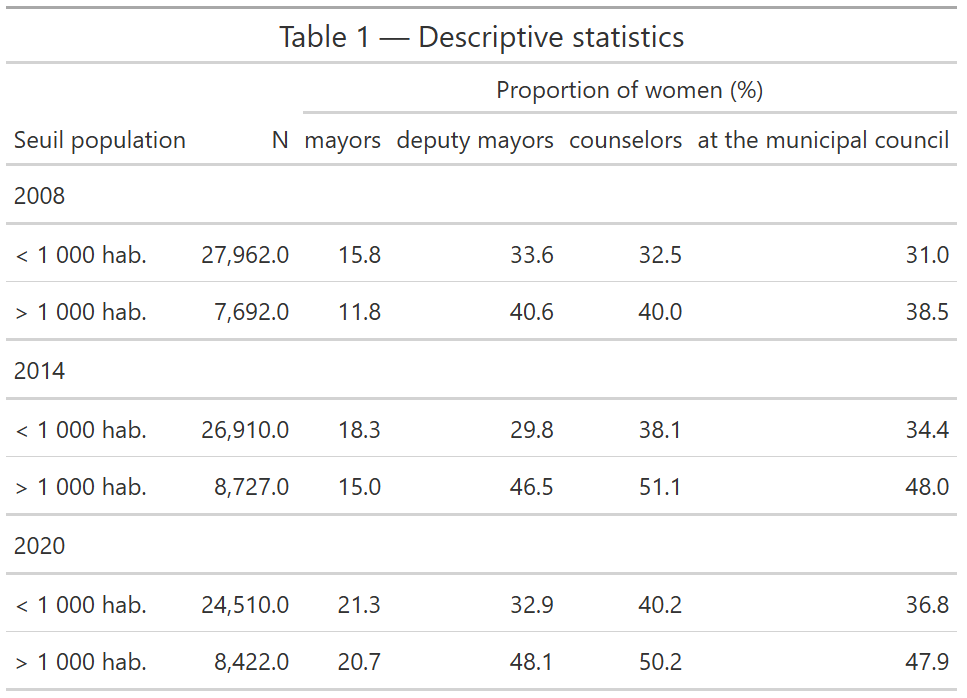
\includegraphics[width=3.28in]{table1_descriptives.png}
\end{figure}

\section{RESULTS}

Over the period considered, we observe a general upward trend across electoral cycles regarding female representation. The share of female councillors, deputy mayors, and mayors increased in all municipalities, above and below the threshold\footnote{Except for the share of female deputy mayors in municipalities $<$1,000 inhabitants which slightly declined between 2008 and 2014 and then back up again in 2020. This might be due to low or misrecording of deputy mayors in 2008.}. This general trend of greater female representation reflects a broader societal change and applies regardless of quota policies. In the following part, we seek to isolate the effect of the quota policy.

\subsection{Locating the glass ceiling on female political representation}

We estimate the impact of quotas along the municipal hierarchy, along councillors, mayors, and the intermediate position of deputy mayors. As seen in table 2 below, quotas increased the proportion of female councillors by 7.2 percentage points in 2014, which is significant at the 1\% level and represents a 20\% increase. However, there is no evidence of a statistically significant effect on the probability of electing a female mayor. This corresponds to documented evidence that zipper quotas substantially increase women's representation among councillors but fail to increase representation at the mayoral level (Lassébie, 2019). This is illustrated by the discontinuity graphs in annex, showing a clear jump in the proportion of female councillors in 2014 (A1), but no discontinuity for mayors in either year (A2).

\begin{figure}[H]
  \centering
  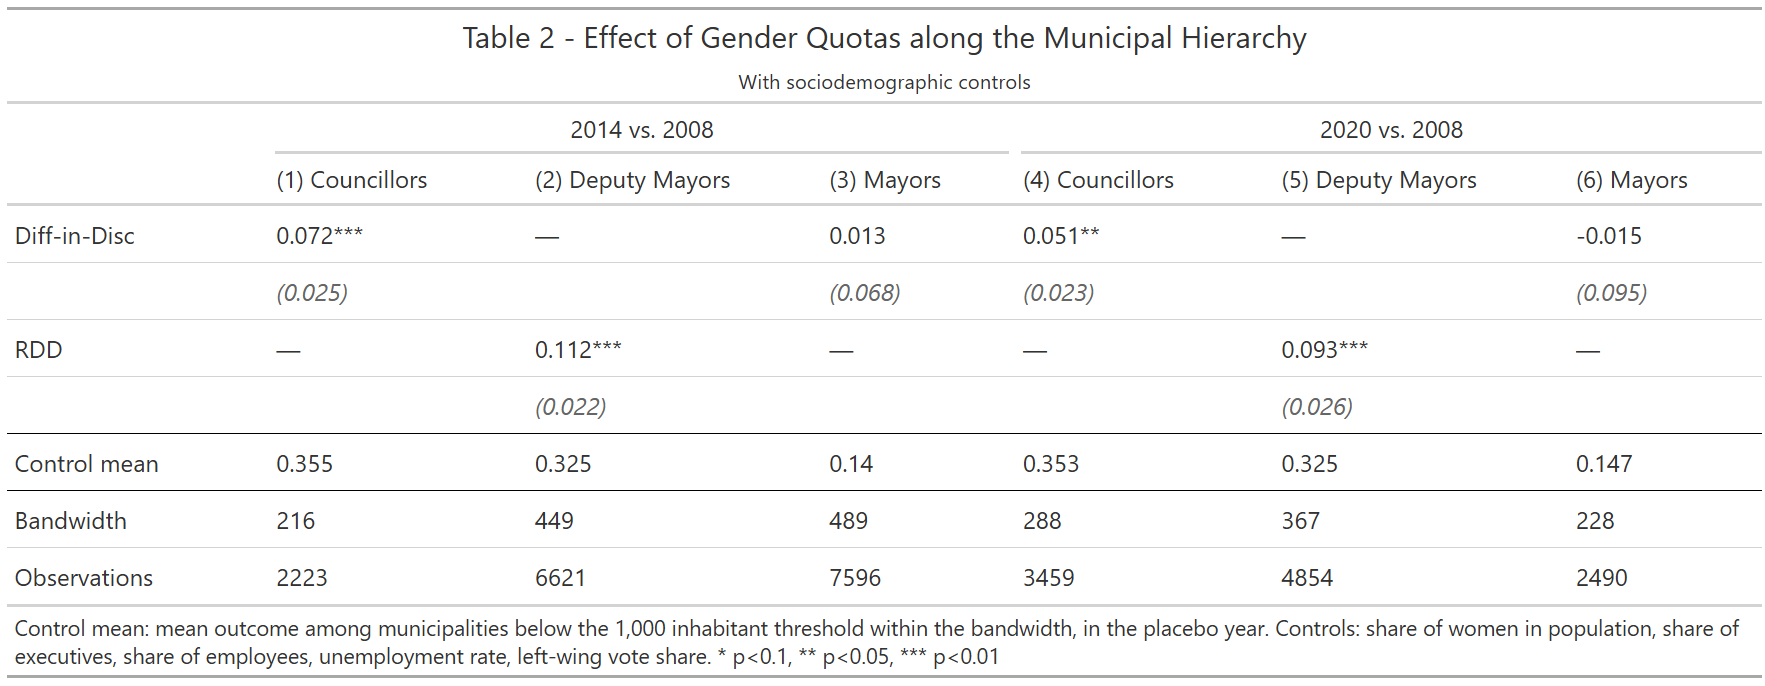
\includegraphics[width=\textwidth]{table2_main_results.png}
\end{figure}

Regarding deputy mayors (A3), municipalities just above the 1,000 inhabitant threshold had a proportion of female deputy mayors 11.2 percentage points higher than municipalities just below (p$<$0.01), which constitutes a statistically significant and larger effect than for councillors, but needs to be interpreted cautiously because it is a simple RD estimate that could also reflect confounding discontinuities at the threshold.

\begin{figure}[H]
  \centering
  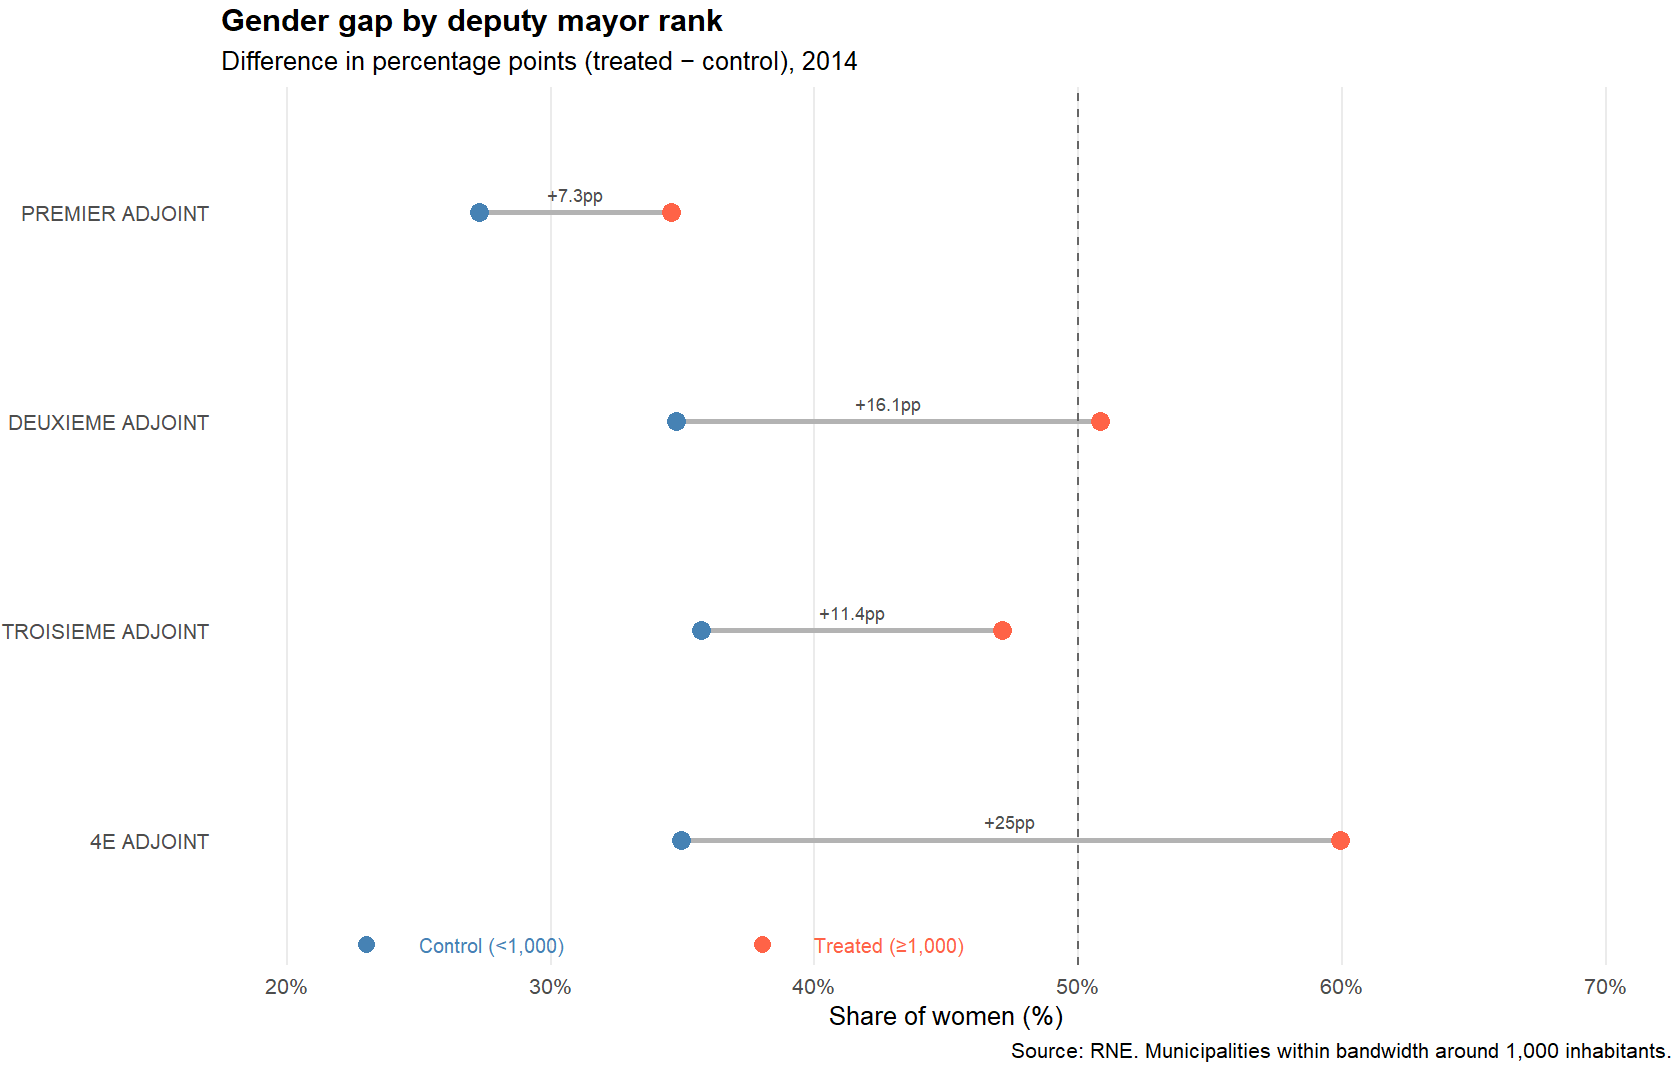
\includegraphics[width=3.6in]{deputy_rank_gap.png}
\end{figure}

Additionally, the adjacent figures nuances the impact of quotas on greater gender balance among deputy mayors. We focus on the first four deputy mayor ranks, which constitute the number of deputies of the vast majority of municipalities within our bandwidth. In that sample, while women are systematically more represented in treated municipalities, parity is only reached at even ranks (2nd, 4th deputy mayors) but not at odd ranks (1st, 3rd). This can illustrate the idea that zipper quotas operate as a binding mechanical constraint, but have a lesser impact on leadership roles where the alternation rule provides no guarantee, as showcased by the low share of female first deputy mayors.

We note that for both councillors and deputy mayors, the 2020 coefficient is smaller than the 2014 one. This could reflect an equalizing effect, since in the first election cycle of 2014 under the new quota policy, treated municipalities experienced a sharp increase in female representation so that the gap between treated and control widens sharply, while in 2020 the shock has been absorbed over two electoral cycles. Additionally, it could showcase the diffusion of progress in gender norms, so that over time the presence of women in politics is increasingly accepted and there is less difference between treated and control municipalities. We cannot conclude that there is an erosion on the effectiveness of quotas over time, as this would require measuring the marginal effect of the second enforcement of quotas, which we cannot reliably estimate.

Therefore, we identify a significant positive effect of quotas on the share of women among councillors and deputy mayors (although differently depending on the rank of the deputy), but not for female mayors. Our findings along the municipal hierarchy echo Lippmann's thesis that gender quotas do not break the glass ceiling, but merely raise it to the level legally set by the quota. The parity law imposes strict gender alternation on candidate lists, generating a significant increase in the share of female councillors and it also mandates parity within the group of deputy mayors, producing also a significant effect at that level. Yet it imposes no constraint on who is at the top position of the list (the mayor position), and for this we find no significant effect on female mayoral representation. This suggests that the glass ceiling indeed lies where the legal constraint intervenes, at the transition between deputy mayors and mayors, indicating that increasing women's representation at lower levels, even intermediate executive ones, does not automatically translate into access to leadership positions.

\subsection{Identifying a role model effect}

We analysed a potential role model effect induced either by the presence of previous female mayor, or by high feminisation among neighbouring municipalities.

\begin{figure}[H]
  \centering
  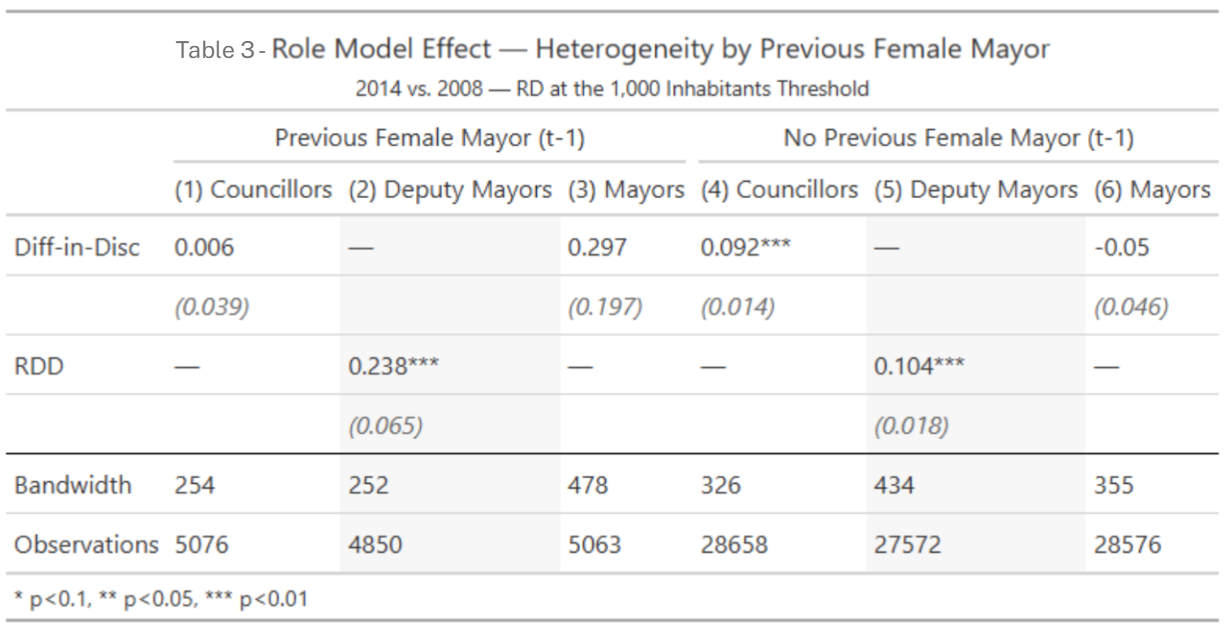
\includegraphics[width=4.36in]{table3_previous_female_mayor.png}
\end{figure}

Table 3 reports the diff-in-disc estimates separately for municipalities with and without a previous mayor. For female councillors, the effect is large and significant in municipalities with no prior female leadership (9.2 pp, p$<$0.01), while it is small and statistically insignificant in municipalities where the previous mayor was a woman. This goes against the role model hypothesis. If anything, it is consistent with an equalising effect of quotas, which have higher effects where women were previously least represented. This might suggest that institutional requirements are stronger than informal role model dynamics. For deputy mayors, both subsamples show a statistically significant positive effect, larger in municipalities with prior female leadership (23.8 vs. 10.4 percentage points). However, these estimates rest on a simple RDD rather than a difference-in-discontinuity design, and may therefore reflect pre-existing differences at the threshold rather than a causal quota effect, so that it can't be interpreted as evidence of role model effect. For mayors, neither estimate is statistically significant, and the larger point estimate in municipalities with previous female leadership might reflect persistence (for instance incumbency effects) rather than a role model mechanism through an additional effect of quotas.

\begin{figure}[H]
  \centering
  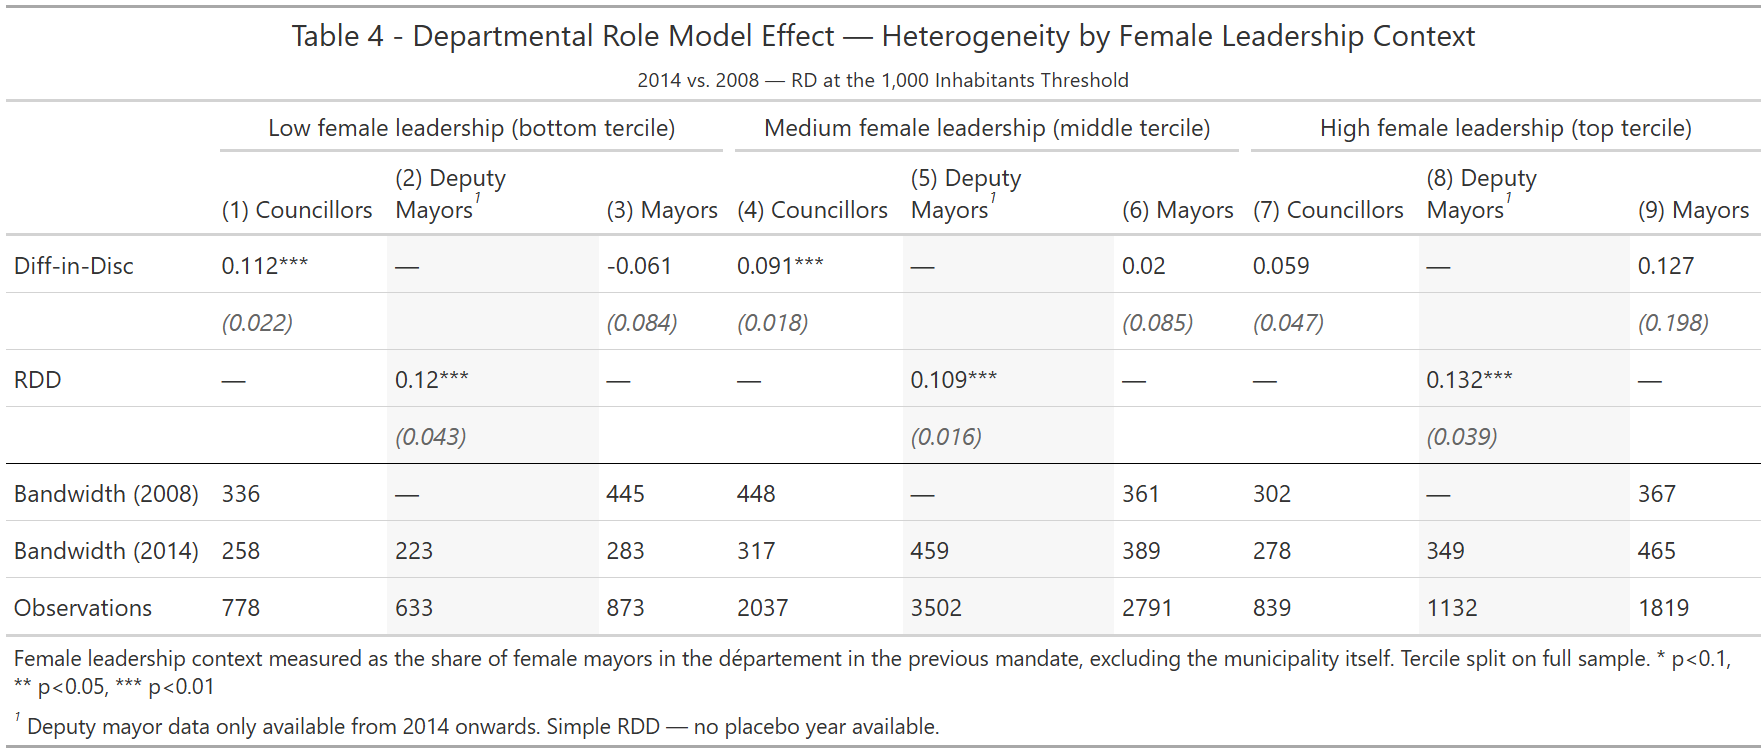
\includegraphics[width=5.29in]{table4_department_terciles.png}
\end{figure}

Table 4 reports estimates across the three terciles of departmental female leadership. Overall, we observe a similarity of coefficients across the three groups at every level. For mayors, neither estimate is statistically significant in either group, consistent with our main results. For deputy mayors, the 3 RD estimates are similar and significant at the 1\% level. For councillors, in low and medium feminisation contexts, the effects are respectively 0.112 and 0.091, significant at the 1\% level, while the estimate in the high female leadership context is smaller and no longer significant. This attenuation reflects the pattern observed for previous female mayors, and could reflect the fact that, in an environment where female political leadership is higher, the quota adds less pressure to increase female representation. Even though we don't observe heterogeneity by feminisation, it is possible that spillover effects could happen at a more granular level between neighbouring municipalities rather than simply in the department, so that checking this would involve using GIS data on municipal proximity.

Taken together, the results provide little support for a role model mechanism amplifying the effects of gender quotas. This could reflect previously mentioned idea that female representation is more impacted by the legal mandate itself, independent of whether pre-existing female leadership has changed local norms. However, this analysis does not constitute a direct test of the role model effect, but rather an additional test to assess whether the quota effect varies systematically with prior female leadership context. The results are therefore informative, but don't allow us to conclude definitively on the lack of role model dynamics.

\section{DISCUSSION}

\subsection{Findings and policy implications}

This paper provides empirical evidence on the effects of quotas across the municipal hierarchy in France, exploiting the 2013 extension of the Parity Law to municipalities above 1,000 inhabitants. We show that the quota significantly increased the share of women among councillors, but produced no significant effect on access to the mayoral level. The effect on deputy mayors is positive and significant, but we document that women are systematically underrepresented in the most senior position, suggesting compliance with the law without fundamentally altering the gender-based hierarchy. Overall, these findings offer support for Lippmann's (2018) thesis that gender quotas do not break the glass ceiling but relocate it to the level left unconstrained by the law.

The absence of heterogeneity by female leadership context further strengthens the interpretation that the quota effect is primarily institutional rather than mediated by local cultural factors. Moreover, the effect of quotas is not amplified in municipalities where women were previously visible in leadership roles, and the larger effects we observe where women were least represented suggests that legal mandates substitute for local role model dynamics. Over the time horizon of our study, institutional rules seem to be the dominant driver of change.

The fact that the glass ceiling sits precisely where the legal constraint is suggests that quotas alone have not been sufficient to incentivize political parties to place women at the top of their lists. This raises the question of whether further legal intervention is warranted, or whether progress at the mayoral level will have to come through slower cultural and educational channels that reshape candidate selection norms within parties.

\subsection{Limitations}

Our study faces some methodological constraints. As with all RDDs, our estimates identify local average treatment effect for municipalities near the 1,000 inhabitants threshold, and thus may not generalise to municipalities further away from the cutoff. For deputy mayors specifically, the absence of pre-2014 data prevents us from implementing a full Difference-in-Discontinuities design, we used simple RDD estimates that may capture confounding discontinuities at the threshold, and should therefore be interpreted with that in mind.

Additionally, the treatment effect captures institutional changes rather than the impact of quotas alone. Indeed, municipalities affected by the lowering threshold simultaneously transitioned from a candidate-centred majoritarian system to a list-based proportional system, which is itself more favourable to women's electoral success (Paxton et al. 2021).

For the role model analysis, our approach does not constitute a direct causal test of the role model effect itself, but rather an assessment of whether the size of the quota-induced jump varies with prior female leadership context.

\subsection{Areas for further research}

Regarding deputy mayors, it would be interesting to link the rank-based differences between genders to the broader literature showing that female elected representatives are often assigned portfolios deemed ``feminine'' (e.g. social affairs, culture) (Achin and Lévêque, 2006). Whether the under-representation of women at senior deputy mayor ranks reflects a similar logic of informal portfolio sorting would be an interesting avenue for further research.

Moreover, the extension of the zipper quota and parity requirement to all French municipalities below 1,000 inhabitants for the 2026 elections (Ministère de l'Intérieur, 2025) constitutes a natural experiment to extend this analysis. It could allow researchers to study the effectiveness of quotas over time and test whether the pattern we document holds across a new wave of treated municipalities. Future work could examine spillover effects at a finer geographic scale and it could also be interesting to track individual careers of female deputy mayors to test whether this position constitutes a pipeline to the mayoral position.

\clearpage
\section*{APPENDIX}

\begin{figure}[H]
  \centering
  \begin{minipage}[t]{0.49\textwidth}
    \centering
    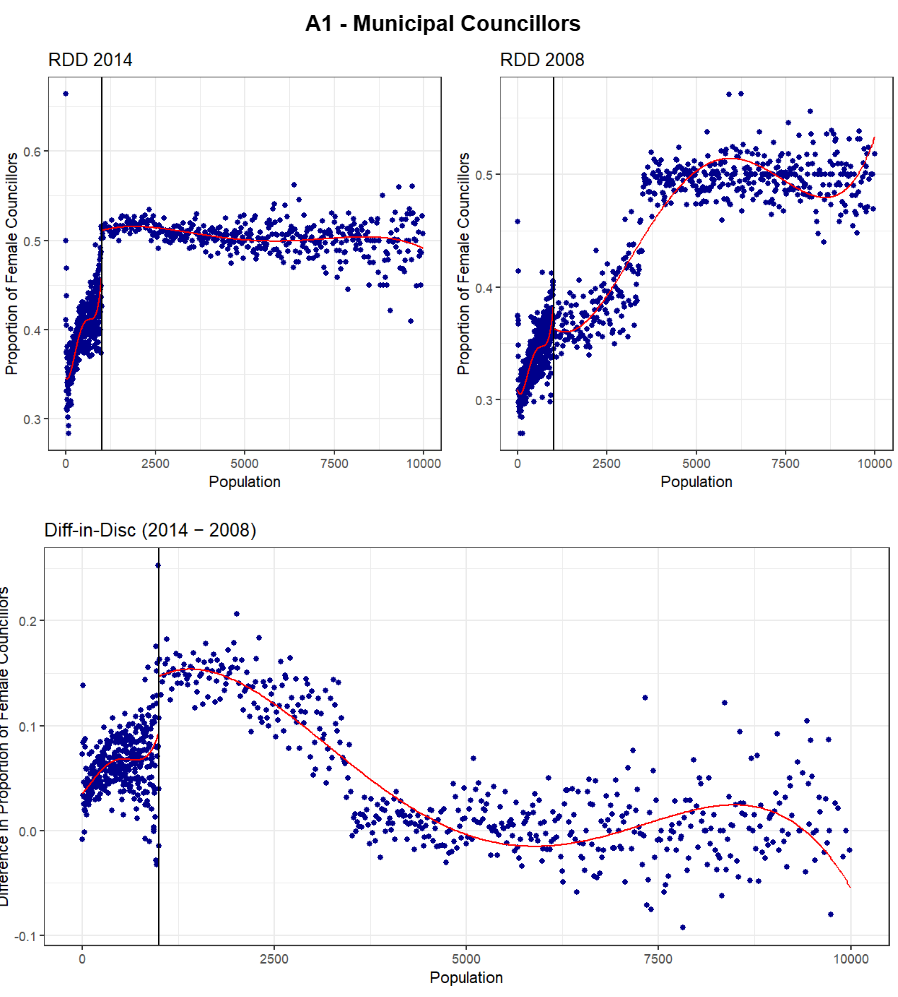
\includegraphics[width=\linewidth]{A1_councillors.png}
  \end{minipage}\hfill
  \begin{minipage}[t]{0.49\textwidth}
    \centering
    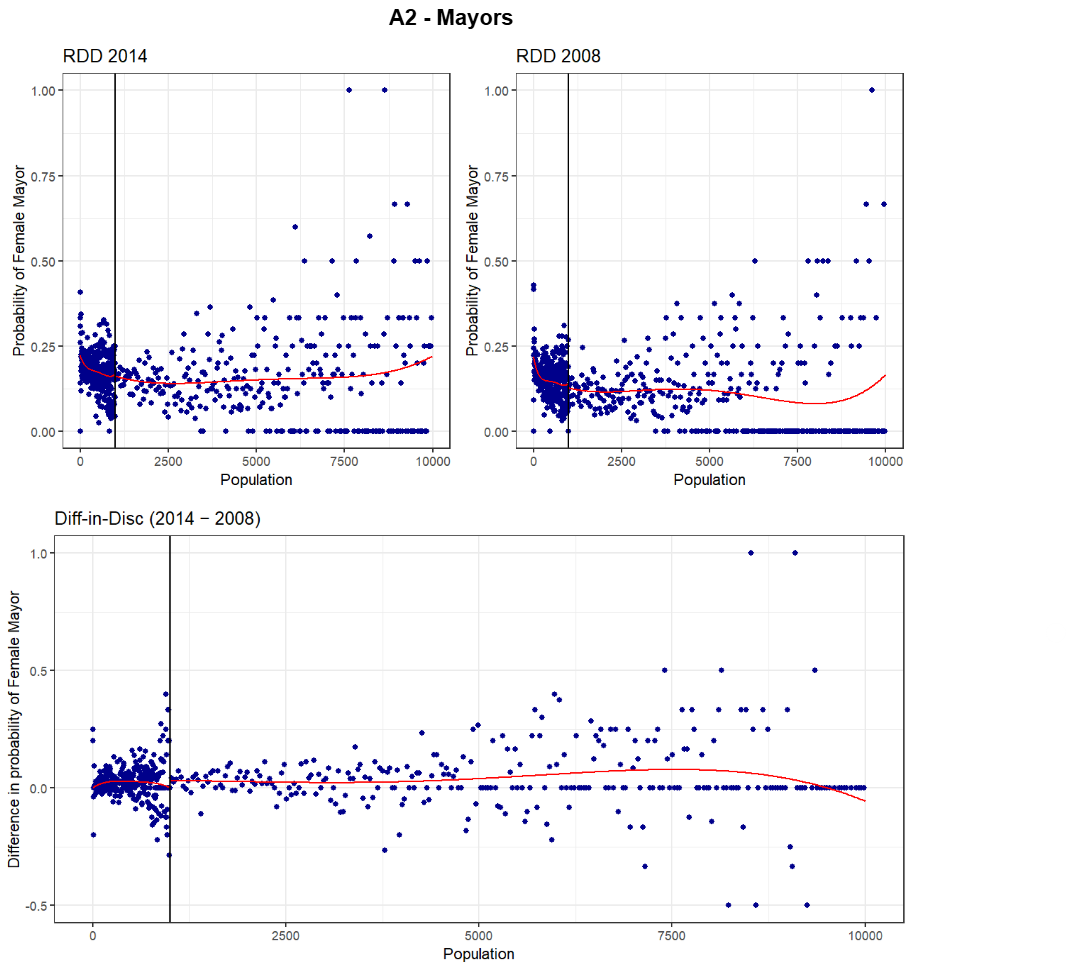
\includegraphics[width=\linewidth]{A2_mayors.png}
  \end{minipage}

  \vspace{1em}
  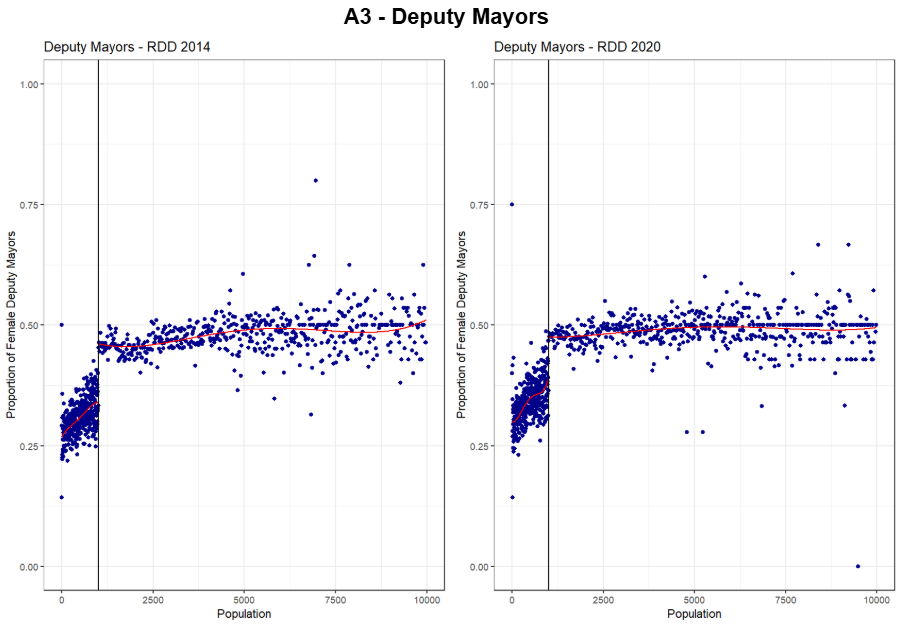
\includegraphics[width=0.6\textwidth]{A3_deputy_mayors.png}
\end{figure}

\section*{Bibliography}

\begin{references}
  \item Achin, C. et Lévêque, S. (2006). III. Femmes et métier politique. Femmes en politique (p. 60-90). La Découverte. \url{https://shs-cairn-info.scpo.idm.oclc.org/femmes-en-politique--9782707147417-page-60?lang=fr}.
  \item Beaman, L., Chattopadhyay, R., Duflo, E., Pande, R., \& Topalova, P. (2009). Powerful women: Does exposure reduce bias? The Quarterly Journal of Economics\textit{,} 124(4), 1497--1540.
  \item Calonico, S., Cattaneo, M. D., \& Titiunik, R. (2014). Robust nonparametric confidence intervals for regression-discontinuity designs. \textit{Econometrica}, \textit{82}(6), 2295-2326.
  \item Gilardi, F. (2015). The temporary importance of role models for women's political representation. American Journal of Political Science, 59(4), 957--970.
  \item Ladam, C., Harden, J. J., \& Windett, J. H. (2018). Prominent role models: High-profile female politicians and the emergence of women as candidates for public office. American Journal of Political Science.
  \item Paxton, P. M., Hughes, M. M., \& Barnes, T. D. (2021). \textit{Women, politics, and power: A global perspective} (Fourth edition). Rowman \& Littlefield.
  \item Spaziani, S. (2022). Can gender quotas break the glass ceiling? Evidence from Italian municipal elections. European Journal of Political Economy, 75, 102171.
  \item Lassébie, J. (2020). ``Gender Quotas and the Selection of Local Politicians: Evidence from French Municipal Elections''. European Journal of Political Economy, vol. 62, p. 101842.
  \item Lippmann, Q. (2018)\textbf{.} Les politiques de quotas en faveur des femmes ont-elles brisé ou surélevé le plafond de verre ? Revue économique, 69(5), 849--867.
  \item Ministère de l'Intérieur. (2025). Municipales 2026 : le mode de scrutin change pour les communes de moins de 1000 habitants. \url{https://www.interieur.gouv.fr/actualites/actualites-du-ministere/municipales-2026-mode-de-scrutin-change-pour-communes-de-moins-de-1-000-habitants}
  \item O'Brien, D. Z., \& Rickne, J. (2016). ``Gender Quotas and Women's Political Leadership''. American Political Science Review, 110(1), 112-126. Science Review, 110(1), 112-126.
  \item Vie publique. (2026). Parité politique hommes-femmes : quels résultats ? \textit{\url{https://www.vie-publique.fr/eclairage/19618-parite-politique-hommes-femmes-quels-resultats}}
\end{references}

\textbf{Datasets}

\begin{references}
  \item Ministère de l'Intérieur. (2025). Répertoire national des élus (RNE). data.gouv.fr. \url{https://www.data.gouv.fr/datasets/repertoire-national-des-elus-1/}
  \item Labatut, V., Févrat, N., Volpi, É., \& Marrel, G. (2025). \textit{BRÉF - Base Révisée des Élu·es de France} [Data set]. Zenodo. \url{https://doi.org/10.5281/ZENODO.14628510}
  \item NosDonnées.fr. (2025). \textit{Résultats des élections présidentielles 2007} [Data set]. data.gouv.fr. \url{https://www.data.gouv.fr/datasets/resultats-des-elections-presidentielles-2007-nd/}
  \item NosDonnées.fr. (2014). \textit{Résultat des élections présidentielles française de 2012 au niveau bureau de vote} [Data set]. data.gouv.fr. \url{https://www.data.gouv.fr/datasets/resultat-des-elections-presidentielles-francaise-de-2012-au-niveau-bureau-de-vote}
  \item Institut national de la statistique et des études économiques (INSEE). (s.d.). \textit{Historiques des populations de référence. Recensement de la population 1968-2023} [Data set]. \url{https://www.insee.fr/fr/statistiques/252260}
  \item Institut national de la statistique et des études économiques (INSEE). (2026). \textit{Recensement de la population -- Population (exploitation complémentaire)} [Data set]. \url{https://catalogue-donnees.insee.fr/fr/catalogue/recherche/DS_RP_POPULATION_COMP}
  \item Institut national de la statistique et des études économiques (INSEE). (2026). \textit{Recensement de la population -- Emploi au lieu de résidence (exploitation principale)} [Data set]. \url{https://catalogue-donnees.insee.fr/fr/catalogue/recherche/DS_RP_EMPLOI_LR_PRINC}
\end{references}

\end{document}
